\documentclass[11pt,a4paper]{article}
\usepackage[utf8]{inputenc}
\usepackage[english]{babel}
\usepackage{amsmath}
\usepackage{amsfonts}
\usepackage{amssymb}
\usepackage{graphicx, wrapfig}
\usepackage[left=2cm,right=2cm,top=2cm,bottom=2cm]{geometry}
\usepackage[hidelinks]{hyperref}
\usepackage{url}
\usepackage{listings}
\usepackage{color}
\usepackage{enumitem}
\usepackage{courier}
\usepackage[bottom]{footmisc}
\usepackage{caption}
\captionsetup{font={small,sf}} % For caption fonts
\captionsetup[sub]{font={small,sf}} % For caption fonts
\usepackage{textcomp}
\usepackage{titling}
\usepackage{tcolorbox}

\setlength{\droptitle}{-2cm}   

\title{\textbf{Assignment 6: Final Programming Project} \\ \Large Advanced Machine Learning Proseminar, Winter Semester 2019-20}
\date{}

\begin{document}
\maketitle

\vspace{-1cm}

\noindent
% Put name and c-number of first member
\textbf{Name/C-number:Raoul Schikora/csav8467}  \\
\textbf{Name/C-number:Oliver Roß/csaq8749}  \\

\section{Answers}

\begin{enumerate}
\item Answer to question 1
	We used a polynomial degree of 3. Extensive testing showed no real progress for a degree of 2. $n>3$ turned out to be not feasible on our laptops or Google Colab in a reasonable amount of time.
\item Answer to question 2 (include 3 figures)
	We trained our LFA Policy Agent with a discount factor $\gamma = 0.9$, a step size $\alpha = 0.02$ and $n = 3$ for 1000 episodes.
	Figures \ref{fig:1} through \ref{fig:3} show the reward per episode during training.
	\begin{figure}
	\begin{center}
		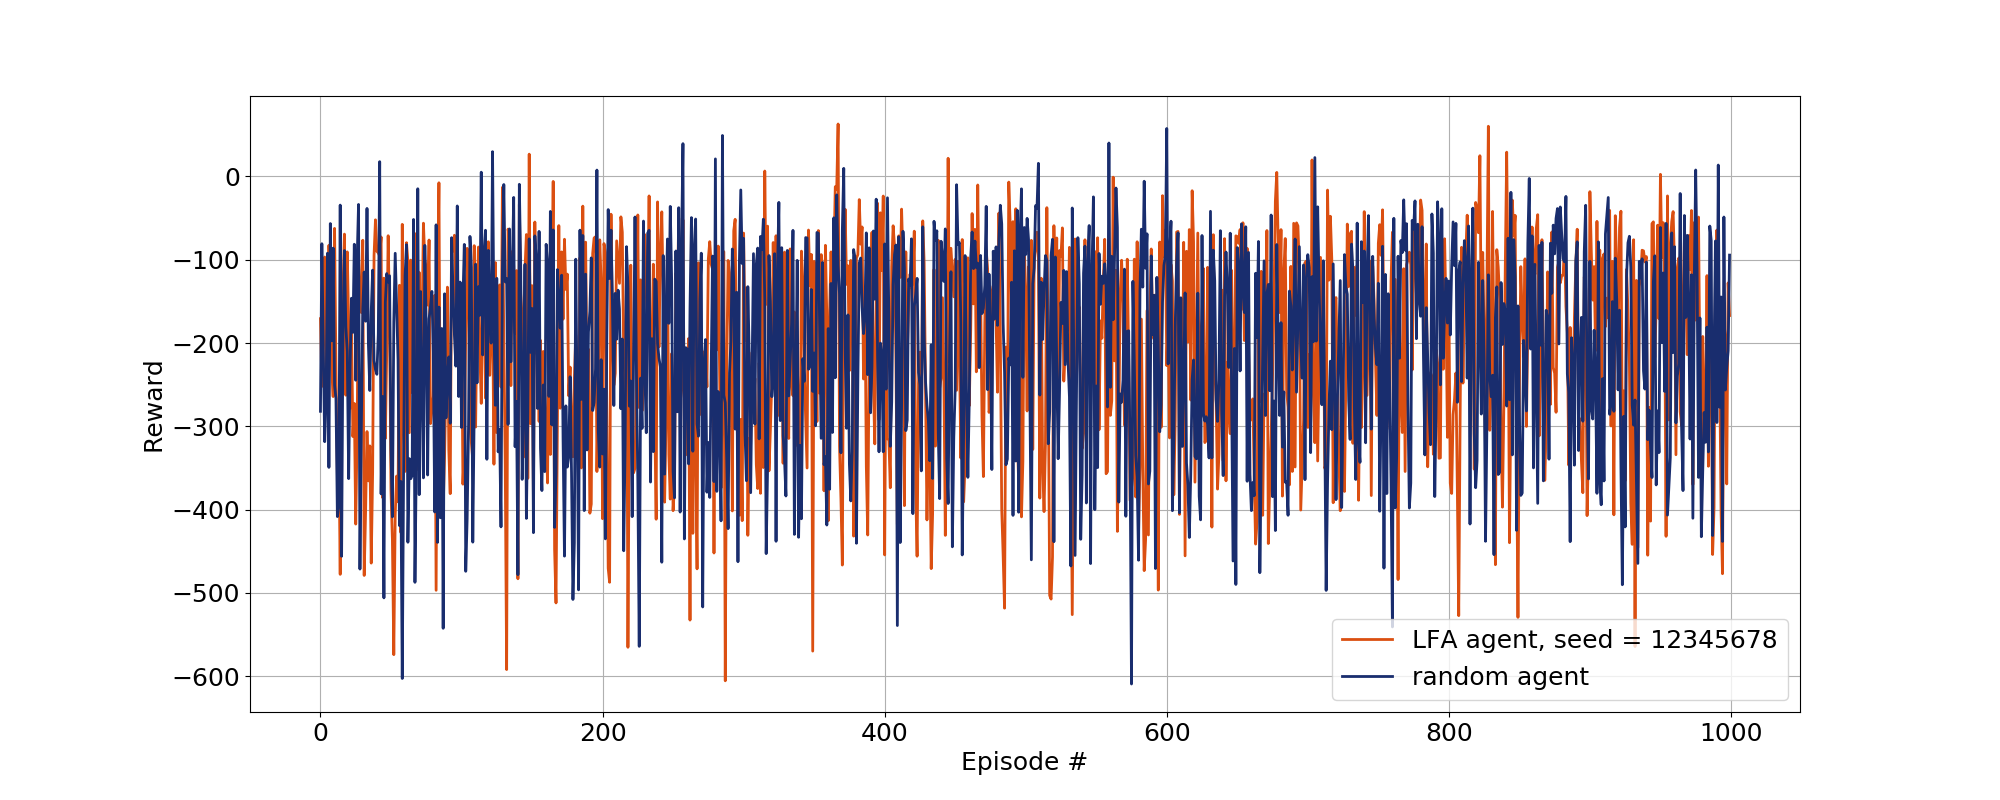
\includegraphics[width = 20cm]{12345678.png}
		\caption{LFA Policy Agent, trained with random seed 12345678. Episode rewards during training.}
		\label{fig:1}
	\end{center}
	\end{figure}

	\begin{figure}
	\begin{center}
		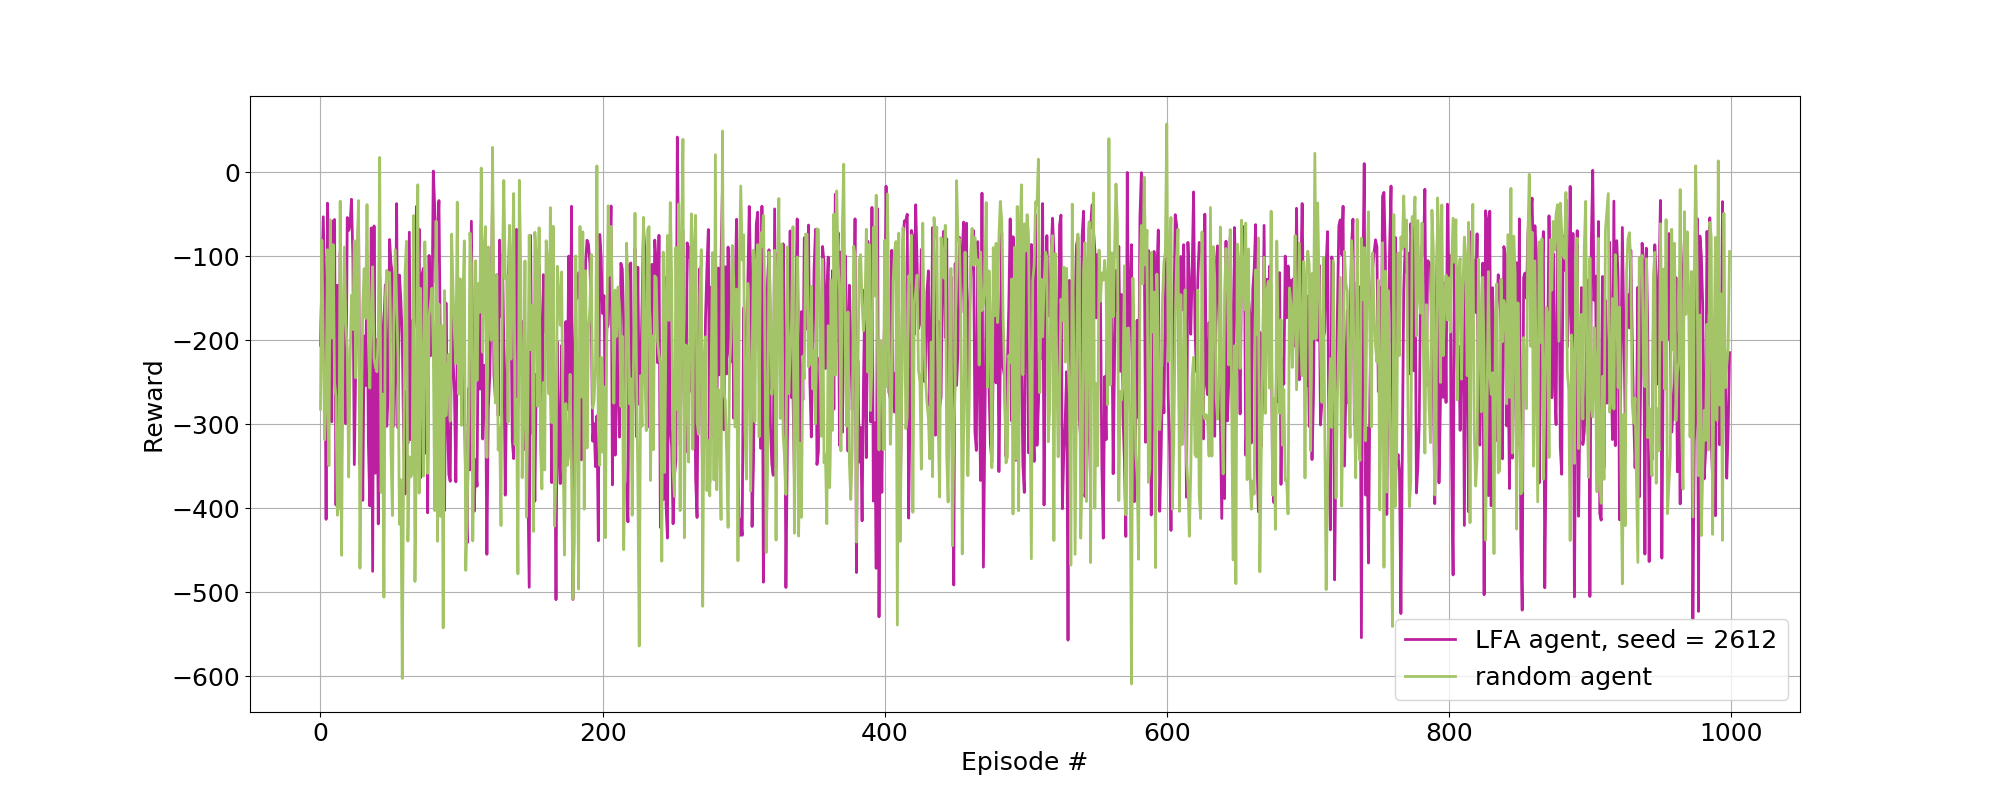
\includegraphics[width = 20cm]{2612.png}
		\
		\caption{LFA Policy Agent, trained with random seed 2612. Episode rewards during training.}
		\label{fig:2}
	\end{center}
	\end{figure}
	\begin{figure}
	\begin{center}
		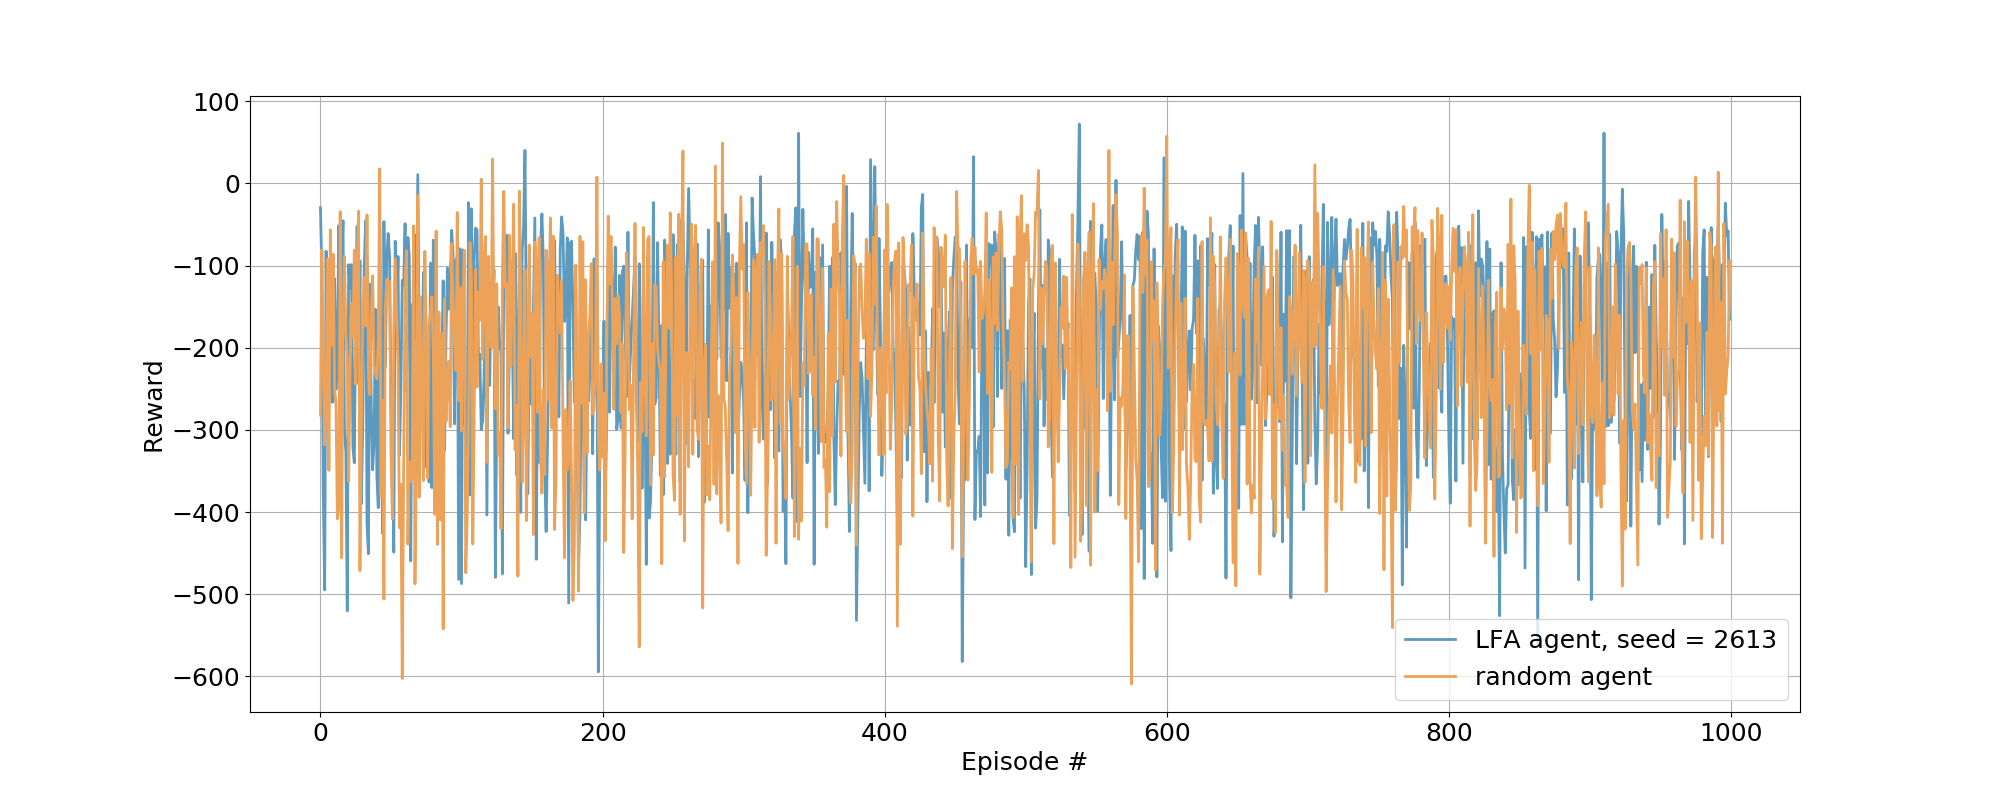
\includegraphics[width = 20cm]{2613.png}
		\caption{LFA Policy Agent, trained with random seed 2613. Episode rewards during training.}
		\label{fig:3}
	\end{center}
	\end{figure}
\item Answer to question 3 
	Our agent didn't perform significantly better than the random agent. When evaluating the policy after it was learned, with deterministically chosen actions (instead of sampled from a gaussian), we observed slightly better performance and less variance compared to the random agent(see figure \ref{fig:4}). \textbf{\textcolor{red}{WHY? EXPLANATION?}}
	\begin{figure}
	\begin{center}
		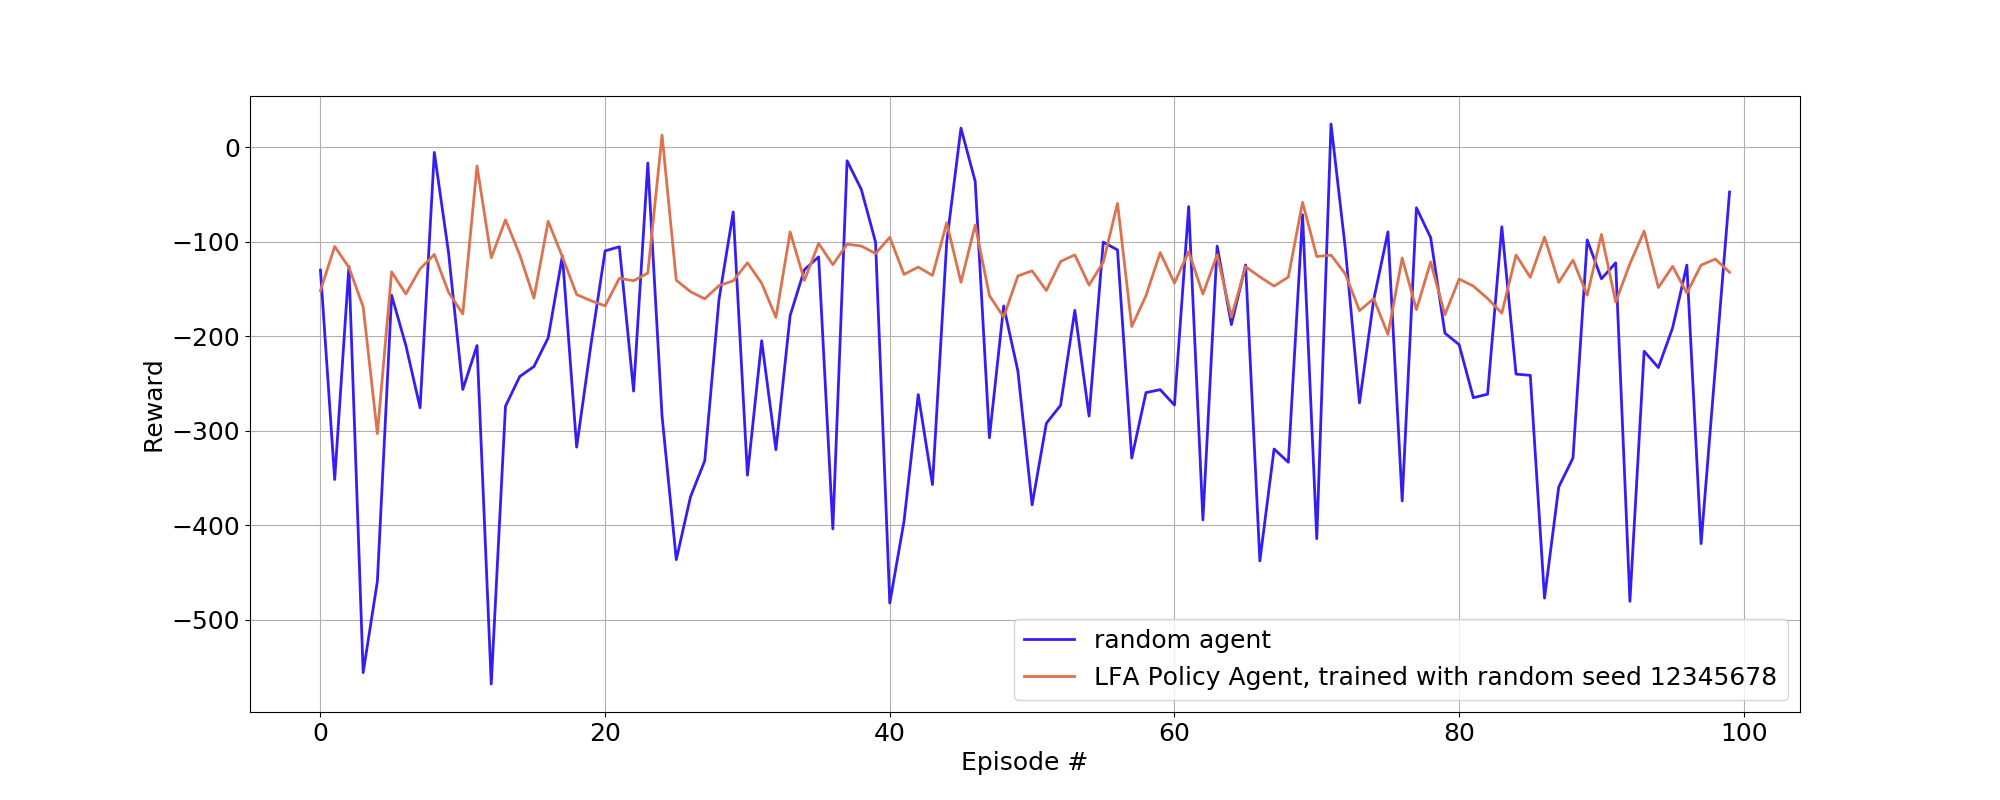
\includegraphics[width = 20cm]{12345678_eval.png}
		\caption{LFA Policy Agent, trained with random seed 12345678. Episode rewards after training.}
		\label{fig:4}
	\end{center}
	\end{figure}
\item Answer to question 4
\item Answer to question 5 (include 3 figures)
\item Answer to question 6
\end{enumerate}

\end{document}
